The previous chapter introduced the concepts of \textit{open-loop} and \textit{closed-loop} control laws, and then dove into techniques for designing open-loop control laws for robots based on optimal control and differential flatness. These techniques are useful for determining control inputs that accomplish different objectives, such as ``move from point A to point B in a minimal amount of time while satisfying some constraints''. Additionally, computing open-loop control laws is often computationally less challenging that computing closed-loop control laws.
However in practice open-loop control is not very robust since observations are not leveraged to update the control input. One solution to this robustness problem is to convert the open-loop control law into a closed-loop control law, typically referred to as \textit{trajectory tracking controllers}. Another solution is to not use any open-loop techniques but rather to directly synthesize a closed-loop control law, for example by performing a \textit{Lyapunov stability analysis}.
This chapter will introduce techniques for synthesizing closed-loop controllers in both of these ways.

\notessection{Closed-loop Motion Planning \& Control}
Recall from the previous chapter that open-loop control laws are defined as a function of time for a given initial condition. In contrast, closed-loop control laws are a function of the \textit{current} state, and therefore are reactive.

\begin{definition}[Closed-loop Control]
If the control law is a function of the state and time, i.e., 
\begin{equation}
\bm{u}(t) = \pi(\x(t), t )    
\end{equation}
then the control is said to be in closed-loop form.
\end{definition}

Closed-loop controllers (also sometimes referred to as \textit{feedback controllers} or \textit{policies}), are much more robust than open-loop controllers. For example, suppose a controller needs to be designed to make a wheeled robot move from point to point. If the model used for open-loop controller design wasn't perfect, if the initial state was not perfectly known, or if external disturbances affected the system (e.g. wheel slipping), then the robot would not exactly reach its desired destination. Alternatively, a closed-loop control law can continuously correct for these errors since it is always taking in new information.

\subsection{Trajectory Tracking}
One common approach to closed-loop control is to simply extend the open-loop control techniques from the previous chapter to include a feedback component. Such an approach consists of two steps:
\begin{enumerate}
    \item Use open-loop control techniques to design a desired trajectory $\x_d(t)$ and corresponding control $\bm{u}_d(t)$.
    \item Design a closed-loop control law that is designed to make sure the system stays close to the desired trajectory.
\end{enumerate}
These controllers are referred to as \textit{trajectory tracking} controllers, and their control law is defined as
\begin{equation}
\bm{u}(t) =  \bm{u}_d(t)+\pi(\x(t)-\x_d(t),t).
\end{equation}
This type of control law is also said to be a ``feedforward plus feedback'' controller. This is because the term $\bm{u}_d(t)$ is an open-loop ``feedforward'' term that attempts to generally make the system follow the desired trajectory, while the term $\pi(\x(t)-\x_d(t),t)$ is a ``feedback'' term that attempts to correct for any errors. 

The previous chapter discussed techniques for solving open-loop control problems to define the desired trajectory, and additionally there are several approaches for designing the feedback component $\pi(\x(t)-\x_d(t),t)$:
\begin{itemize}
  \item \textit{Geometric} approaches generally leverage some sort of insight about the system and are therefore hard to discuss in general settings. They are also typically difficult to derive theoretical guarantees for. 
  \item \textit{Linearization} based approaches typically linearize nonlinear dynamics models about points along the desired trajectory. These linearized models are then used to design linear controllers (e.g. linear quadratic regulators). For some nonlinear systems, instead of linearizing about specific points it possible to \textit{feedback linearize} the system. This essentially means that the non-linearities can be exactly ``canceled'' out such that the system can be considered linear. Linear control theory can then be applied to design a feedback control scheme.
  
  \item \textit{Non-linear control} techniques also exist which do not rely on linearization. These approaches are also heavily system dependent, but one common tool for non-linear control is based on \textit{Lyapunov} theory.

  \item \textit{Optimization-based} feedback control laws can also be designed. These approaches often leverage optimal control theory, some of which was presented in the previous chapter. One common optimization-based approach for closed-loop control is known as \textit{model predictive control} (MPC).
\end{itemize}

\subsubsection{Trajectory Tracking for Differentially Flat Systems}
For differentially flat systems linearization based approaches to designing trajectory tracking controllers are particularly useful\cite{Levine2009}. In fact, every flat system can be linearized via dynamic feedback and a coordinate change to yield a dynamical system of the form
\begin{equation} \label{eq:diff_flat_linearized}
    \z^{(q+1)} = \bm{w}, 
\end{equation}
where $\z^{(q+1)}$ is the $q+1$-th order derivative of the flat outputs $z$ and $q$ is the degree of the flat output space (i.e. the highest order of derivatives of the flat output that are needed to describe system dynamics), and $\bm{w}$ is a modified ``virtual'' input term.

The set of ODEs \eqref{eq:diff_flat_linearized} are \textit{linear}, which means that techniques from linear control theory can be applied to design a control law for $\bm{w}$. In particular, for trajectory tracking problems suppose a reference flat output trajectory $\z_d(t)$ has been defined which corresponds to the virtual input $\bm{w}_d(t)$. Let the error between the actual flat output and desired flat output be defined as $\bm{e}(t) = \z(t) - \z_d(t)$ and consider a closed-loop control law of the form
\begin{equation}
w_i(t) = w_{i,d}(t) - \sum_{j=0}^q k_{i,j} e_i^{(j)}(t),
\end{equation}
where $(\cdot)_i$ denotes the $i$-th component of the vector, $e^{(j)} = \z^{(j)} - \z_d^{(j)}$ is the $j$-th order derivative of the error, and $k_{i,j}$ are called controller \textit{gains}.
The application of this control law to the system \eqref{eq:diff_flat_linearized} will result in \textit{closed-loop dynamics} of the form
\begin{equation*}
\begin{split}
\z^{(q+1)} &= \bm{w}_d - \sum_{j=0}^q K_j \bm{e}^{(j)}, \\
\end{split}
\end{equation*}
where $K_j$ is a diagonal matrix with $i$-th diagonal element $k_{i,j}$. Since $\z_d^{(q+1)} = \bm{w}_d(t)$ this can be simplified to give the closed-loop error dynamics:
\begin{equation}
\begin{split}
\bm{e}^{(q+1)} + \sum_{j=0}^q K_j \bm{e}^{(j)} = 0. \\
\end{split}
\end{equation}
This set of linear ODEs describes the dynamics of the error, and many classical techniques from linear control theory can be used to choose the gains $k_{i,j}$ that will guarantee this system is \textit{stable}. Having stable error dynamics means that the error will decay to zero, which in this case means the system will track the desired trajectory.

\begin{example}[Extended Unicycle Trajectory Tracking] \label{ex:trajtrack}
\theoremstyle{definition}
Consider the dynamically extended unicycle model
\begin{equation}
\begin{split}
\dot{x}(t) &= v \cos(\theta(t)), \\
\dot{y}(t) &= v \sin(\theta(t)), \\
\dot{v}(t) &= a(t), \\
\dot{\theta}(t) &= \omega(t),
\end{split}
\label{robot_eq_dyn}
\end{equation}
where the two inputs are the acceleration $a(t)$ and the rotation rate $\omega(t)$. This system is differentially flat with flat outputs $x$ and $y$ and order $q=1$. It can therefore be expressed as:
\begin{equation*}
\ddot{\z} = \begin{bmatrix} \ddot{x} \\ \ddot{y} \end{bmatrix} = \underbrace{\begin{bmatrix} \cos(\theta) & -V\sin(\theta) \\ \sin(\theta) & V\cos(\theta) \end{bmatrix}}_{:=J} \begin{bmatrix} a \\ \omega \end{bmatrix} := \begin{bmatrix} w_1 \\ w_2 \end{bmatrix},
\end{equation*}
and a trajectory tracking controller can be defined as
\begin{equation*}
\begin{split}
    w_1 &= \ddot{x}_d - k_{px}(x - x_d)- k_{dx}(\dot{x} - \dot{x}_d),\\
    w_2 &= \ddot{y}_d - k_{py}(y-y_d)- k_{dy}(\dot{y}-\dot{y}_d),\\
\end{split}
\end{equation*}
where $(\cdot)_d$ represents a term associated with the desired trajectory. The control inputs $a(t)$ and $\omega(t)$ can then be computed by solving the linear system
\begin{equation*}
J\begin{bmatrix} a \\ \omega \end{bmatrix} = \begin{bmatrix} w_1 \\ w_2 \end{bmatrix},
\end{equation*}
assuming that $J$ is full rank.
\end{example}


\subsection{Closed-loop Control}
Trajectory tracking is just one example of closed-loop control, which assumes the existence of a desired trajectory for which to track. As previously discussed, one way of computing the desired trajectory is by solving an open-loop optimal control problem. However, in the context of optimal control, modifying an open-loop optimal control with feedback is not always the most desirable option. Instead, it may be preferred to just directly solve a closed-loop optimal control problem to obtain an optimal policy $\bm{u}^* = \pi(\x(t),t)$. Techniques for solving closed-loop optimal control problems typically are based on either the Hamilton-Jacobi-Bellman equation or dynamic programming.

Another common closed-loop control problem is to drive to or stabilize the system about a particular state (often called \textit{regulation}). For systems with linear dynamics models the most controller for regulation problems is called the \textit{linear quadratic regulator}. However, for nonlinear systems, stabilizing closed-loop controllers are commonly designed through \textit{Lyapunov analysis}\cite{SlotineLi1991}.

\subsubsection{Lyapunov-based Control}
A Lyapunov stability analysis is a common tool for analyzing the stability of nonlinear systems. This analysis is based on the definition of a Lyapunov function, which can be thought of as a measure of the ``energy'' of the system. Similar to mechanical systems, if the energy does not increase in time then the system is considered stable\footnote{Note there are more technical definitions of stability, but for simplicity these will not be discussed here}.

The most challenging part of a Lyapunov stability analysis is finding a suitable Lyapunov function, and for many complex systems this may be extremely difficult. However, one of the advantages of the method is that it provides nice theoretical guarantees regarding the stability of the system, and is applicable to any system of interest.

\begin{example}[Pose Stabilization] \label{ex:pose}
\theoremstyle{definition}
\cite{AicardiCasalinoEtAl1995} Consider a robot that is modeled by the unicycle robot model (differential drive robot model) represented graphically in Figure \ref{fig:posecartesian}
\begin{equation} \label{eq:posecartesian}
\begin{split}
\dot{x}(t) &= v(t) \cos\theta(t), \\
\dot{y}(t) &= v(t) \sin\theta(t), \\
\dot{\theta}(t) &= \omega(t),
\end{split}
\end{equation}
where the control inputs are the robot speed $v$ and the rotational rate $\omega$. The objective is to design a closed-loop controller that will drive the robot the origin (i.e. $x=0$, $y=0$, $\theta = 0$).

\begin{marginfigure}
\centering
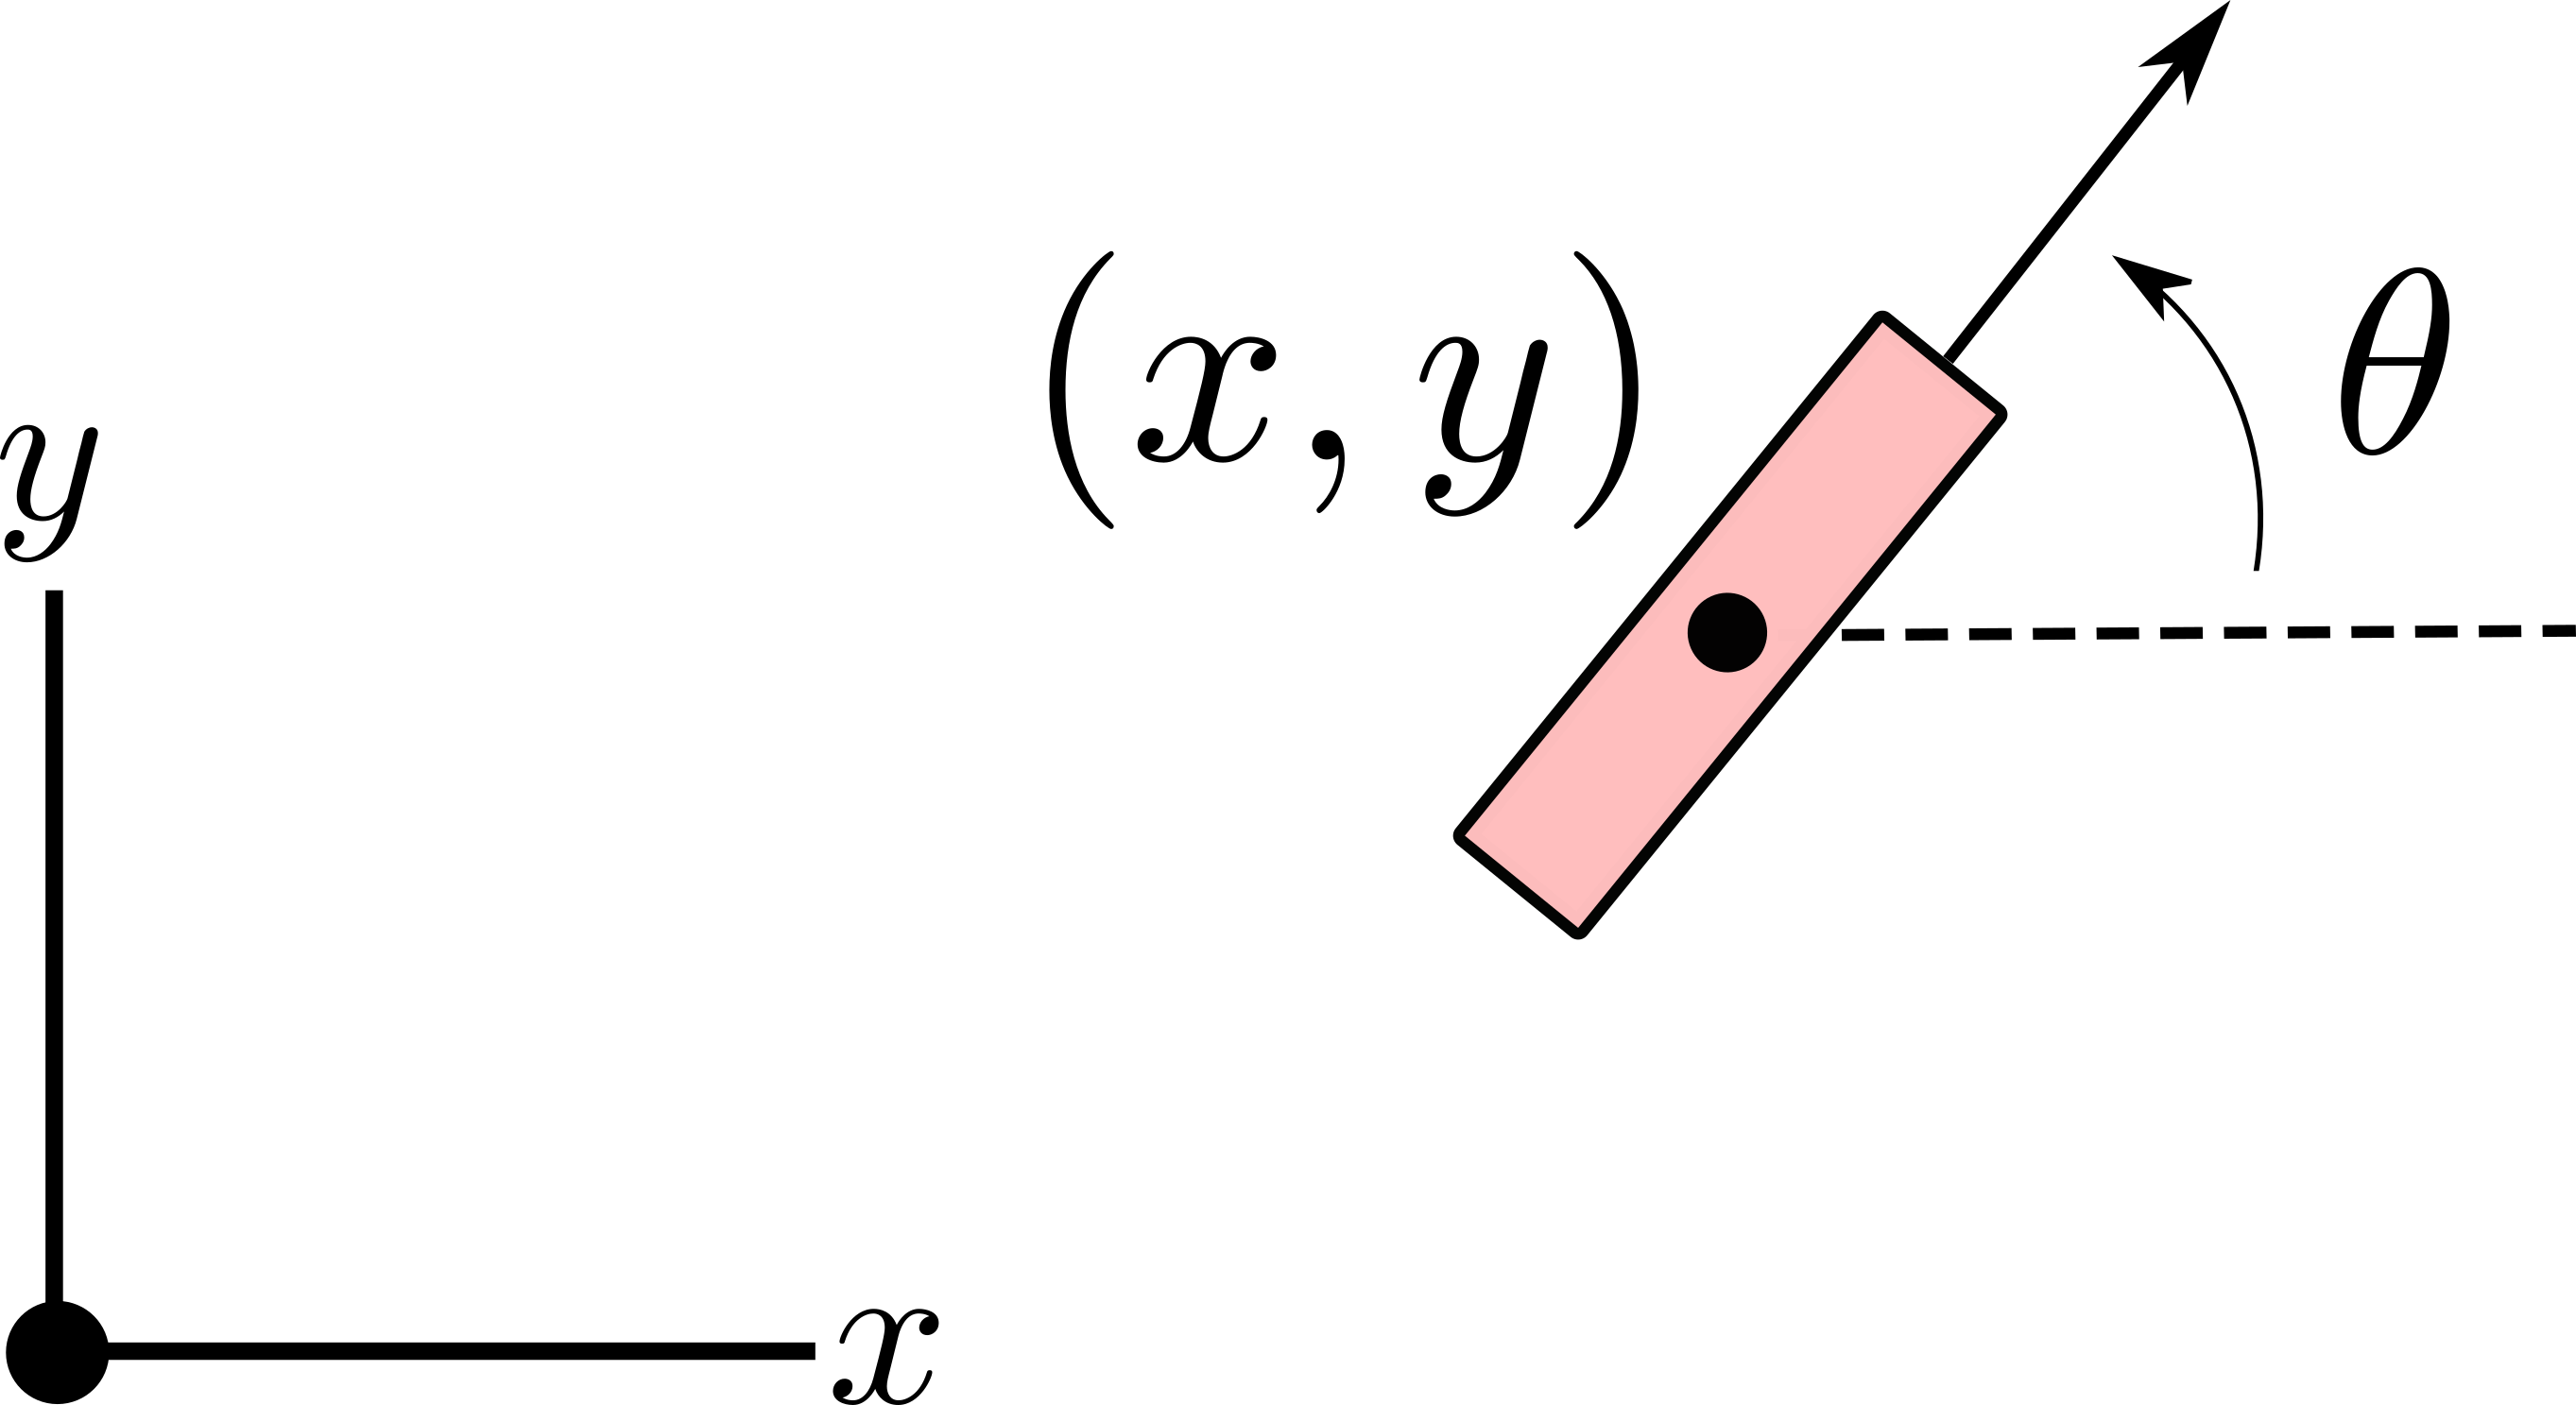
\includegraphics[width=0.9\textwidth]{tex/figs/ch04_figs/unicycle_cartesian.png}
\caption{Pose stabilization of a unicycle robot in Cartesian coordinates.}
\label{fig:posecartesian}
\end{marginfigure}

To make the controller design easier the dynamics will be alternatively expressed in polar coordinates. This can be accomplished by defining
\begin{equation} \label{eq:polarcoord}
\begin{split}
\rho &= \sqrt{x^2+y^2}, \\
\alpha &= \mathrm{atan2}(y, x) - \theta + \pi, \\
\delta &= \alpha + \theta,
\end{split}
\end{equation}
where $\rho$ is the Euclidean distance to the origin, $\alpha$ is the heading angle with respect to the line from the robot to the origin, and $\delta$ is the angle between the $x$-axis and the line from the robot to the origin. These coordinates are graphically shown in Figure \ref{fig:polarcoord}.
\begin{marginfigure}
\centering
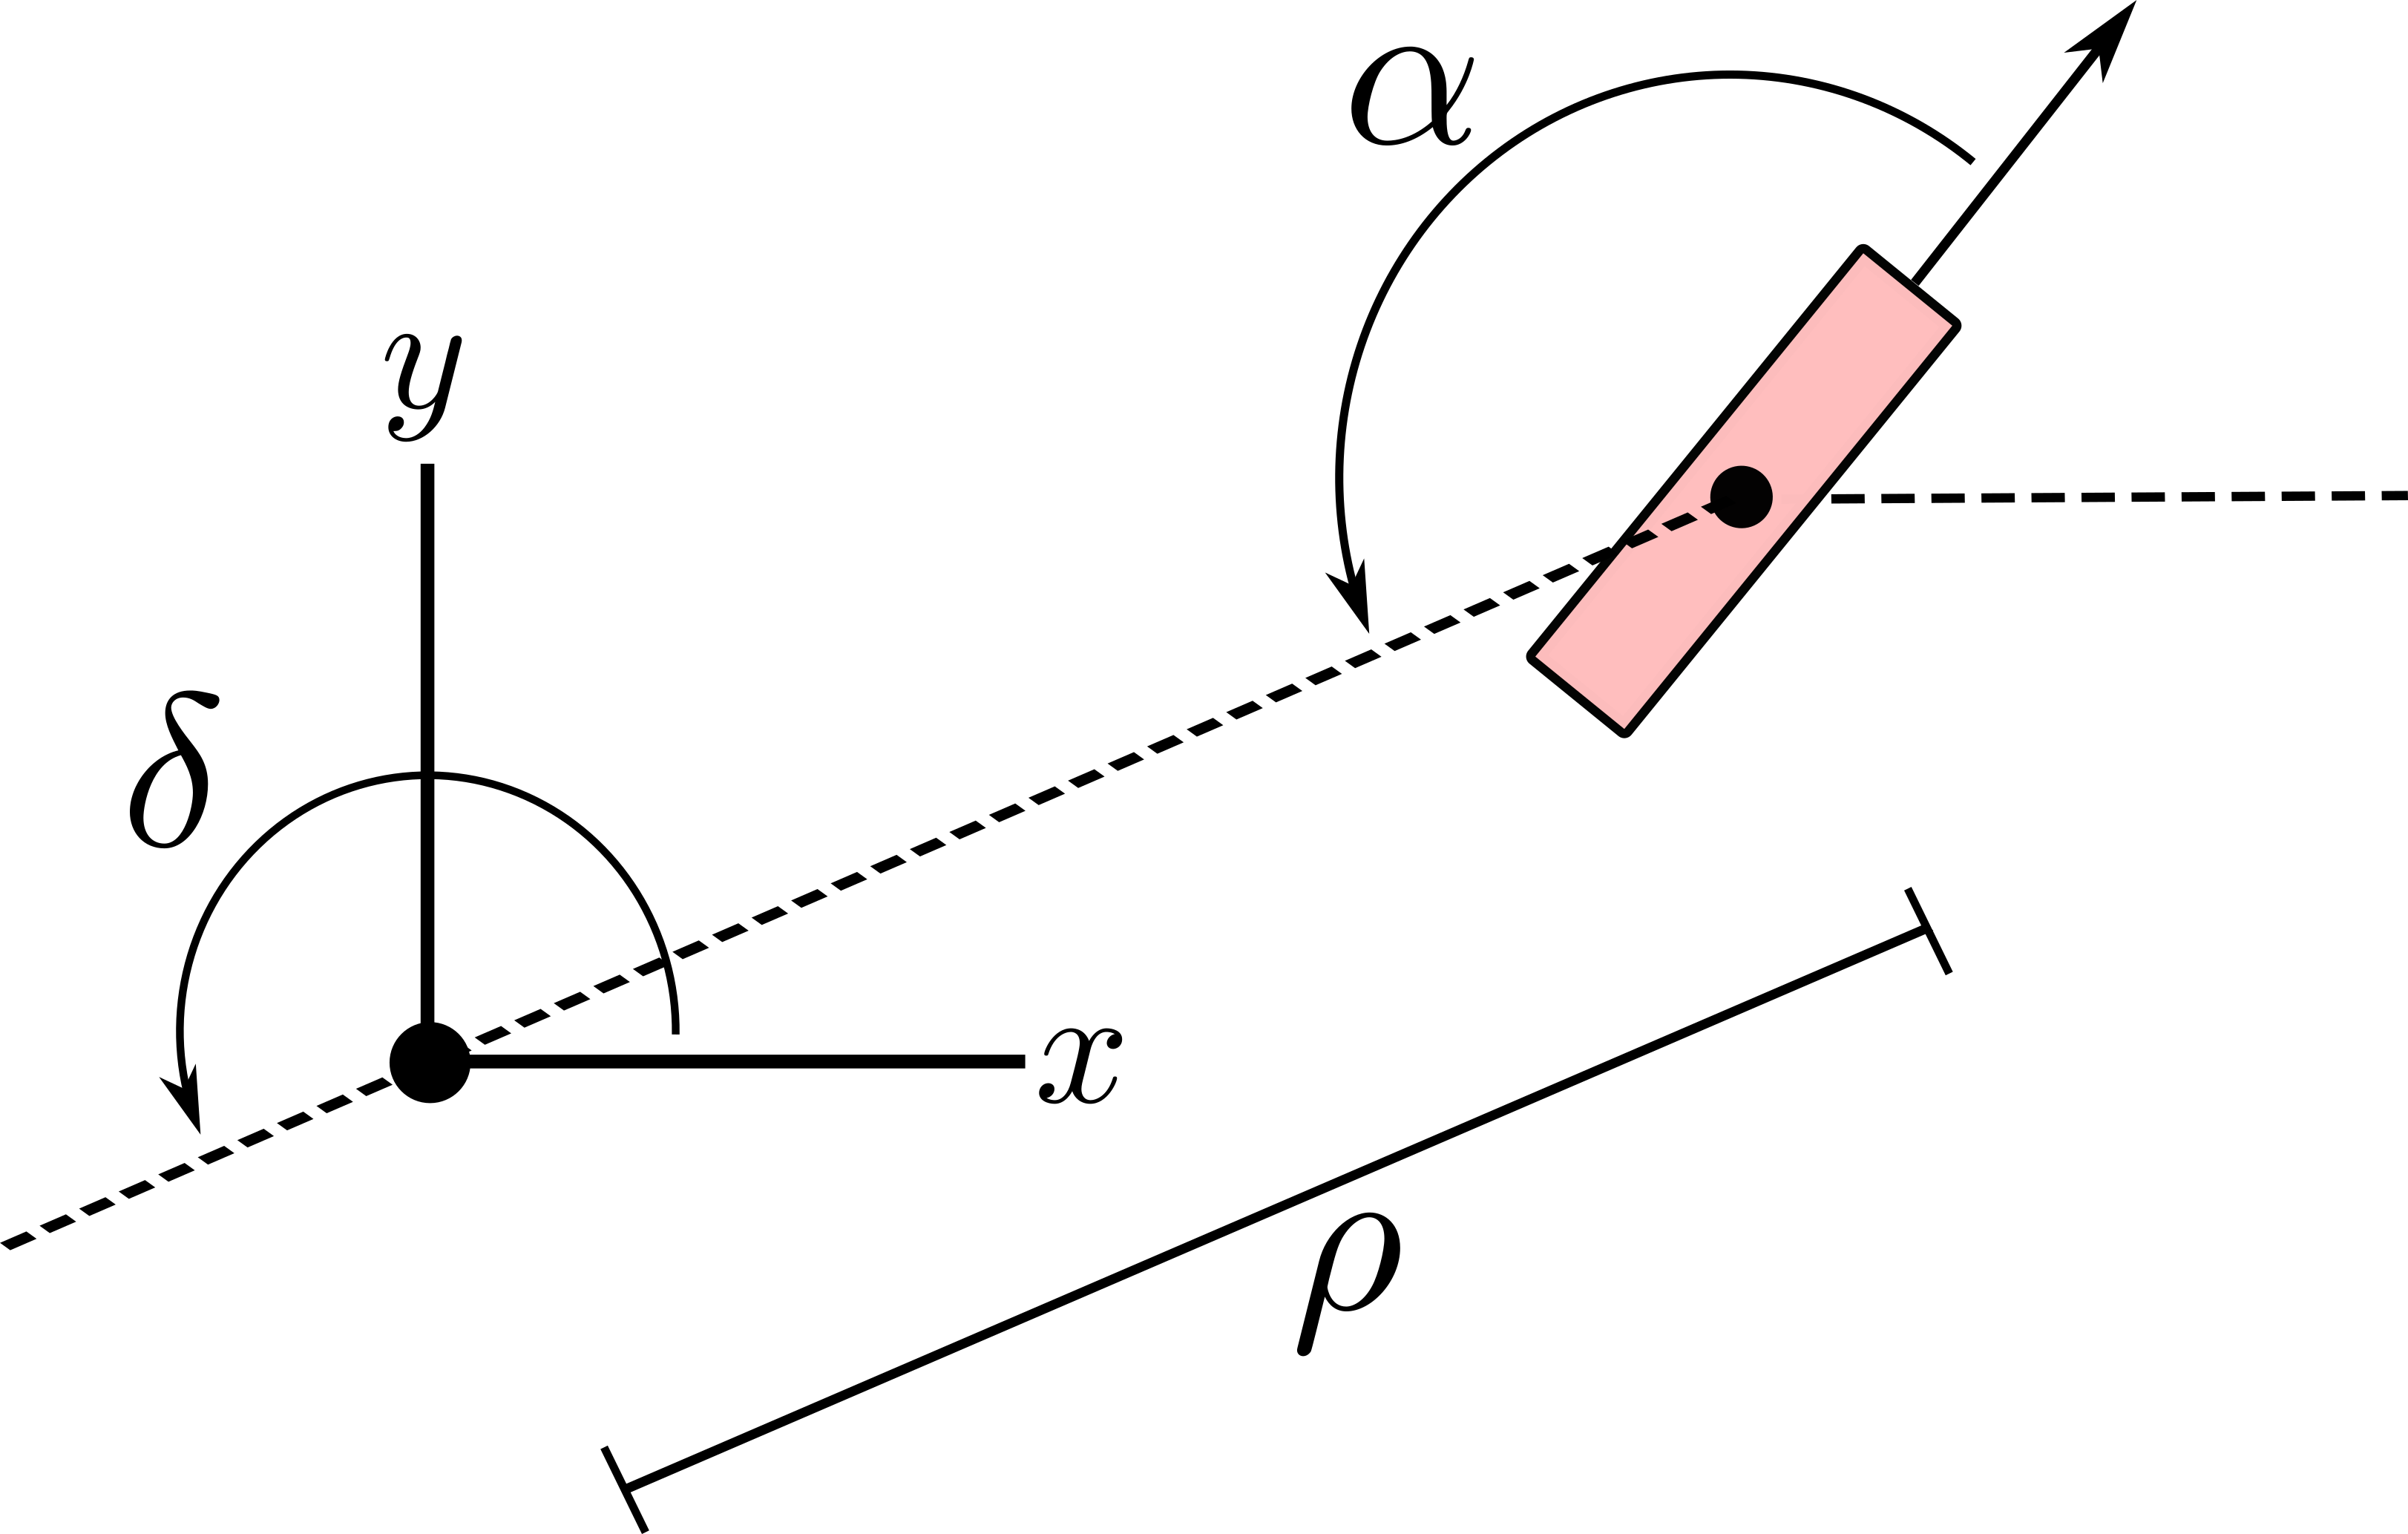
\includegraphics[width=0.95\textwidth]{tex/figs/ch04_figs/unicycle_polar.png}
\caption{Pose stabilization of a unicycle robot using polar coordinates.}
\label{fig:polarcoord}
\end{marginfigure}
Using the newly defined polar coordinates, the dynamics equations \eqref{eq:posecartesian} can be equivalently expressed as
\begin{equation} \label{eq:posepolar}
\begin{split}
\dot{\rho}(t) &= -v(t) \cos\alpha(t), \\
\dot{\alpha}(t) &= \frac{v(t) \sin\alpha(t)}{\rho(t)} - \omega(t), \\
\dot{\delta}(t) &= \frac{v(t) \sin \alpha(t)}{\rho(t)}. \\
\end{split}
\end{equation}

By expressing the dynamics in polar form, a Lyapunov stability analysis can now be easily performed. Consider the following \textit{candidate} Lyapunov function:
\begin{equation}
V(\rho, \alpha, \theta) = \frac{1}{2} \rho^2 + \frac{1}{2} (\alpha^2 + k_3 \delta^2),
\end{equation}
and consider the following closed-loop control law:
\begin{equation} \label{eq:poselaw}
\begin{split}
v &= k_1 \rho \cos \alpha,
\\
\omega &= k_2 \alpha + k_1 \frac{\sin \alpha \cos \alpha}{\alpha}(\alpha + k_3 \delta),
\end{split}
\end{equation}
where $k_1, k_2, k_3>0$.

The candidate Lyapunov function is quadratic and therefore is positive everywhere, $V \geq 0$, and is equal to zero only at the origin with $\rho = 0$, $\alpha = 0$, $\delta=0$. Therefore, if it is possible to show that along \textit{all} closed-loop system trajectories the Lyapunov function is \textit{decreasing} ($\dot{V} < 0$), then it can be guaranteed that the system will converge to the origin! To show that the Lyapunov function decreases along trajectories of the system, begin by taking the derivative of $V$:
\begin{equation*}
\dot{V} = \rho \dot{\rho} + \alpha \dot{\alpha} + k_3 \delta \dot{\delta}.
\end{equation*}
This quantity can now be shown to decrease along \textit{all} closed-loop trajectories by substituting in the dynamics equations \eqref{eq:polarcoord} with the closed-loop control law as defined by \eqref{eq:poselaw}:
\begin{equation*}
\begin{split}
\dot{V} &= \rho \dot{\rho} + \alpha \dot{\alpha} + k_3 \delta \dot{\delta}, \\
&= - \rho v \cos\alpha + \alpha \big(\frac{v \sin\alpha}{\rho} - \omega \big) +  \frac{k_3 \delta v \sin \alpha}{\rho}, \\
&= -k_1 \rho^2 \cos^2 \alpha  - k_2 \alpha^2, \\
\end{split}
\end{equation*}
where in the last line the control laws were substituted in for $v$ and $\omega$ and algebraically simplified. Note that since $k_1$ and $k_2$ have been chosen to be strictly positive, this function must be strictly negative for all values of $\rho$ and $\alpha$! Therefore this Lyapunov stability analysis has theoretically proven that the system under the closed-loop control law \eqref{eq:poselaw} will converge to the origin.
\end{example}

\subsection{Exercises}
Both exercises for this chapter can be found in the online repository:

\vspace{\baselineskip}

\url{https://github.com/PrinciplesofRobotAutonomy/AA274A_HW1}.

\subsubsection{Pose Stabilization}
Complete \textit{Problem 2: Pose Stabilization}, where you will implement the Lyapunov-based pose controller for the unicycle robot described in Example \ref{ex:pose}.

\subsubsection{Trajectory Tracking}
Complete \textit{Problem 3: Trajectory Tracking}, where you will implement the differential flatness-based trajectory tracking controller for the extended unicycle robot described in Example \ref{ex:trajtrack}.